\documentclass[../../../../main.tex]{subfiles}

\begin{document}

\section*{京大理科 数学 1975 表紙・配点・概略}

\begin{itemize}
    \item 所要時間: 90分 / 150分
\end{itemize}

\subsection*{各問のメモ・解答概要}
\begin{enumerate}
    \item チームの勝ち数 $n-1, n-2, \dots, 0$ より第 $k$ 位のチームは $n-k$ 勝。$k$ に関する数学的帰納法により証明する。
    \item (1) AM-GM不等式より $\frac{x+1}{2} \ge \sqrt{x}$。(2) 不等式の両辺を $[0,k]$ で積分し、置換積分を用いて与式 $< 1$ を示す。
    \item 条件式 $2\beta = \alpha + \gamma$ と $\sin^2\beta = \sin\alpha \sin\gamma$ から $\sin^2\frac{\alpha+\gamma}{2} + \sin^2\frac{\alpha-\gamma}{2} = 0$ を導き、$(\alpha, \beta, \gamma) = ((n+k)\pi, n\pi, (n-k)\pi)$ ($n, k \in \mathbb{Z}$) を得る。
    \item $\vec{d} = \vec{PA} + \vec{PB} + \vec{PC} = 3(\vec{g} - \vec{p})$ より $|\vec{d}| = 3|\vec{PG}|$。直線 $OG$ と定円の交点のうち $G$ と $O$ に関して反対側の点を $P$ としたときに最大となる。
    \item $S = n-2 - \sum_{i=1}^n \frac{1}{a_i} > 0$ を最小にする $(n, a_1, \dots, a_n)$ を探す。$n=3$ で $(a_1, a_2, a_3) = (2, 3, 7)$ のとき最小値 $\frac{1}{42}$ となる。
    \item 直角二等辺三角形 $ABC$ に中心 $O(t,t)$ の単位円 $T$ が辺と2点で交わる条件から $x=1/t$ の範囲を求めて面積 $S$ を $x$ で表し、$x = \frac{3}{4}\sqrt{2}$ で最大となることを示す。
\end{enumerate}

\newpage

\section*{第1問}

\noindent
[\textbf{解}] 1チームの勝ち数は、$n-1, n-2, \dots, 1, 0$ の $n$ 通りしかないので、題意から、第 $k$ 位のチーム $A_k$ は $n-k$ 勝していることになる ($k=1, 2, \dots, n$)。

\noindent
以下、題意の成立を $k$ についての帰納法で示す。

\begin{enumerate}
    \item[$1^\circ$] $k=1$ の時\\
    1位のチームは $n-1$ 勝、つまり他の全てのチームに勝っており、成立。

    \item[$2^\circ$] $k=i$ での成立を仮定 ($i=1, 2, \dots, n-1$)\\
    $k=i+1$ の時、仮定から、$A_{i+1}$ は $A_1 \sim A_i$ のチームに負けており、少なくとも $i$ 回負けている。従って、$n-(i+1)$ 勝するには残りの全ての試合に勝つことになるから、$k=i+1$ でも成立。
\end{enumerate}

\noindent
以上から示された。

\newpage

\section*{第2問}

\noindent
[\textbf{解}]
\begin{enumerate}
    \item[(1)] $x \ge 0$ から AM-GMより
    \[
    \frac{x+1}{2} \ge \sqrt{x} \quad \dots \text{①}
    \]

    \item[(2)] ①から $[0, k]$ の時
    \[
    \sqrt{x}\left(1 - \frac{x}{k}\right)^k \le \frac{1}{2}(x+1)\left(1 - \frac{x}{k}\right)^k
    \]
    両辺同じ区間で積分し、与式左辺を $A$ として
    \[
    A < \frac{1}{2}\int_0^k (x+1)\left(1 - \frac{x}{k}\right)^k dx
    \]
    $t = 1 - \frac{x}{k}$ とおくと $\frac{dt}{dx} = -\frac{1}{k}$、$x : 0 \to k$ で $t : 1 \to 0$ だから
    \begin{align*}
    A &< \frac{1}{2} \int_1^0 \{1 + k(1-t)\} t^k \cdot (-k) dt \\
    &= \frac{1}{2} k \int_0^1 \{(1+k)t^k - k t^{k+1}\} dt \\
    &= \frac{1}{2} k \left[ t^{k+1} - \frac{k}{k+2} t^{k+2} \right]_0^1 \\
    &= \frac{1}{2} k \cdot \frac{2}{k+2} = \frac{1}{1 + 2/k} < 1 \quad (\because k \in \mathbb{N})
    \end{align*}
\end{enumerate}

\newpage

\section*{第3問}

\noindent
[\textbf{解}] 題意から
\[
\begin{cases}
2\beta = \alpha + \gamma \quad \dots \text{①} \\
\sin^2\beta = \sin\alpha \sin\gamma \quad \dots \text{②}
\end{cases}
\]
①を②に代入
\begin{align*}
\sin^2 \frac{\alpha+\gamma}{2} &= 2\sin\frac{\alpha}{2}\cos\frac{\alpha}{2} \sin\frac{\gamma}{2}\cos\frac{\gamma}{2} \\
&= \frac{1}{2} \left[ \sin\frac{\alpha+\gamma}{2} + \sin\frac{\alpha-\gamma}{2} \right] \left[ \sin\frac{\alpha+\gamma}{2} - \sin\frac{\alpha-\gamma}{2} \right]
\end{align*}
$t = \frac{\alpha+\gamma}{2}, s = \frac{\alpha-\gamma}{2}$ とおく。
\[
\sin^2 t + \sin^2 s = 0 \quad \dots \text{③}
\]
$\sin t, \sin s \in \mathbb{R}$ から、③が成立するのは
\[
\sin t = \sin s = 0
\]
\[
\therefore \frac{\alpha+\gamma}{2} = n\pi, \quad \frac{\alpha-\gamma}{2} = k\pi \quad (n, k \in \mathbb{Z})
\]
の時である。解いて
\[
\alpha = (n+k)\pi, \quad \gamma = (n-k)\pi
\]
①に代入して
\[
\beta = n\pi
\]
従って、題意のようになるのは、$n, k \in \mathbb{Z}$ として
\[
(\alpha, \beta, \gamma) = ((n+k)\pi, n\pi, (n-k)\pi)
\]

\newpage

\section*{第4問}

\noindent
[\textbf{解}] 点 $X$ の位置ベクトルを $\vec{x}$ で定める。$\vec{d} = \vec{PA} + \vec{PB} + \vec{PC}$ とし、$G$ を $\triangle ABC$ の重心とすると
\begin{align*}
\vec{d} &= \vec{a} + \vec{b} + \vec{c} - 3\vec{p} \\
&= 3(\vec{g} - \vec{p})
\end{align*}
\[
\therefore |\vec{d}| = 3|\vec{g} - \vec{p}| = 3|\vec{PG}|
\]
したがって、定円の中心 $O$、直線 $OG$ と定円の交点のうち、$G$ と $O$ に関して反対側のものを $E$ として、$P = E$ の時 与式は最大。

\newpage

\section*{第5問}

\noindent
[\textbf{解}]
\[
\begin{cases}
2 \le a_1 \le a_2 \le \dots \le a_n \quad \dots \text{①} \\
S = n-2 - \displaystyle\sum_{i=1}^n \frac{1}{a_i} > 0
\end{cases}
\]

\begin{enumerate}
    \item[(i)] $n=3$ の時
    \[
    S = 1 - \left( \frac{1}{a_1} + \frac{1}{a_2} + \frac{1}{a_3} \right)
    \]
    だから、$S > 0$ をみたすうち、逆数和を max にするような $a$ の組をもとめれば良いが、$S$ は $2 \le x$ で単調減少なことから、$S$ ちいさくして考える。

    \begin{enumerate}
        \item[$1^\circ$] $a_1 = 2$ の時\\
        $\frac{1}{a_2} + \frac{1}{a_3} < \frac{1}{2}$ をみたすうち逆数和を max にする $a_2, a_3$ をかんがえる。$a_2, a_3 \ge 2$ から、$(a_2-2)(a_3-2) > 4$ だから、
        \[
        (a_2, a_3) = (3, 7), (4, 5) \text{ 又は } a_2 \ge 5
        \]
        なので、もとめる組は $(a_1, a_2, a_3) = (2, 3, 7)$。

        \item[$2^\circ$] $a_1 = 3$ の時\\
        $\frac{1}{a_2} + \frac{1}{a_3} < \frac{1}{3} \iff (a_2-3)(a_3-3) > 9$ をみたす逆数和を max にする $a_2, a_3$ をもとめる。$(a_2, a_3) = (4, 13), (5, 8), (6, 7)$ or $a_2 \ge 7$ で、明らかに $1^\circ$ の時より和が小さい。
    \end{enumerate}
    以上から、もとめるのは $(a_1, a_2, a_3) = (2, 3, 7)$。

    \item[(ii)] $n \ge 5$ の時、$a_i = 2\ (i=1, 2, \dots, n)$ とすることになり
    \[
    S = n-2 - \frac{n}{2} = \frac{1}{2}(n-4) > 0
    \]
    となって $S$ は最小値をとる。$n$ をうごかした時、これは明らかに $n=5$ で最小値をとる！以下 $n \le 4$ として考える。$n=1$ の時 $S$ は明らかに負だから不適。よって $n=4$ をしらべる。$\frac{1}{x}$ が $2 \le x$ で単調増加なことと $2 = a_1 = a_2 = a_3 = a_4$ の時 $S=0$ であることから、$a_1 = a_2 = a_3 = 2, a_4 = 3$ の時 $\min S = 2 - \left(\frac{1}{2} + \frac{1}{2} + \frac{1}{2} + \frac{1}{3}\right) = \frac{1}{6}\ (>0)$ をとる。
\end{enumerate}

\noindent
以上から、
\[
\begin{cases}
n \ge 5 \text{ の時 } n=5, a_i=2 \text{ で } \min S = \frac{1}{2} \\
n = 4 \text{ 〃 } a_1=a_2=a_3=2, a_4=3 \text{ で } \min S = \frac{1}{6} \\
n = 3 \text{ 〃 } (a_1, a_2, a_3)=(2,3,7) \text{ で } \min S = \frac{1}{42}
\end{cases}
\]
よって、$S$ を min にするのは
\[
n=3, \quad (a_1, a_2, a_3) = (2, 3, 7)
\]
の時。

\newpage

\section*{第6問}

\noindent
[\textbf{解}] $A$ を原点、$B(2,0), C(0,2)$ とする $xy$ 平面で考える。又、$O(t,t)\ (0 < t)$ とおき題意の円を $T$ とおく。
\[
T : (x-t)^2 + (y-t)^2 = 1
\]
\[
BC : x+y = 2
\]

\begin{center}
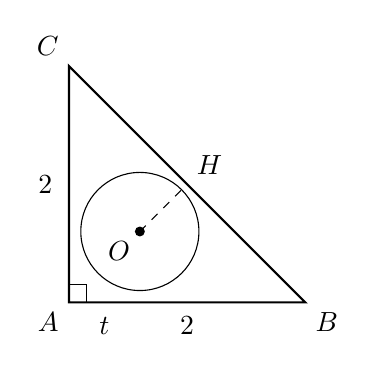
\begin{tikzpicture}[scale=1.5]
    \draw[thick] (0,2) node[above left]{$C$} -- (0,0) node[below left]{$A$} -- (2,0) node[below right]{$B$} -- cycle;
    \draw (0,0) -- (0,0.15) -- (0.15,0.15) -- (0.15,0);
    \coordinate (O) at (0.6,0.6);
    \draw (O) circle (0.5);
    \fill (O) circle (1.2pt) node[below left]{$O$};
    \draw[dashed] (O) -- (1.0,1.0) node[above right]{$H$};
    \node at (0.3,-0.2) {$t$};
    \node at (1.0,-0.2) {$2$};
    \node at (-0.2,1.0) {$2$};
\end{tikzpicture}
\end{center}

\begin{enumerate}
    \item[(i)] $T$ と $x$ 軸の交点は $x^2 - 2tx + 2t^2 - 1 = 0$ の2実解\\
    $T$ と $y$ 軸の交点は $y^2 - 2ty + 2t^2 - 1 = 0$ の2実解\\
    $T$ と $BC$ の交点は $2x^2 - 4x + 2t^2 - 4t + 3 = 0$ の2実解\\
    だからこれらが $0 \le x \le 2, 0 \le y \le 2$ に2実解を持つ条件を考えて、

    \begin{align*}
    &\begin{cases}
    \text{軸}: 0 < t < 2 \\
    \text{端}: 2t^2 - 1 \ge 0, \ 2t^2 - 4t + 3 \ge 0 \\
    \text{判}: t^2 - (2t^2 - 1) > 0
    \end{cases}
    \quad \wedge \quad
    \begin{cases}
    \text{軸}: 0 < 1 < 2 \\
    \text{端}: 2t^2 - 4t + 3 \ge 0, \ 2t^2 - 4t + 3 \ge 0 \\
    \text{判}: 4 - 2(2t^2 - 4t + 3) > 0
    \end{cases}
    \\
    &\iff
    \begin{cases}
    0 < t < 2 \\
    \frac{\sqrt{2}}{2} \le t < 1
    \end{cases}
    \quad \wedge \quad
    2 - \sqrt{2} < t < 2 + \sqrt{2} \\
    &\iff \frac{\sqrt{2}}{2} \le t < 1
    \end{align*}
    よって、$x = 1/t$ だから、$1 \le x < \sqrt{2}$。

    \item[(ii)] (i)の時、$T$ の中心と $x, y$ 軸、$BC$ との距離は各々
    \[
    t, \quad t, \quad |\sqrt{2} - \sqrt{2}t|
    \]
    だから、$F(t)$ が右図斜線部の面積を表すことから、

    \begin{center}
    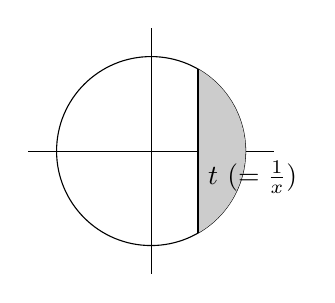
\begin{tikzpicture}[scale=1.2]
        \draw (0,0) circle (1);
        \draw (-1.3,0) -- (1.3,0);
        \draw (0,-1.3) -- (0,1.3);
        \draw[thick] (0.5,-0.866) -- (0.5,0.866);
        \fill[gray!40] (0.5,-0.866) arc (-60:60:1) -- cycle;
        \draw (0.5,-0.866) -- (0.5,0.866);
        \node[below right] at (0.5,0) {$t\ (= \frac{1}{x})$};
    \end{tikzpicture}
    \end{center}

    \[
    S = \pi - 2F\left(\frac{1}{x}\right) - F(\sqrt{2} - x)
    \]

    \item[(iii)] (ii)から
    \begin{align*}
    \frac{dS}{dx} &= +4 \sqrt{1 - \frac{1}{x^2}} \cdot \frac{1}{x^2} - 2\sqrt{1 - (\sqrt{2}-x)^2} \\
    &= 2 \left[ \sqrt{2 - x^2} - \sqrt{1 - (\sqrt{2}-x)^2} \right] \\
    &= 2 \frac{-2\sqrt{2}x + 3}{\sqrt{2-x^2} + \sqrt{1 - (\sqrt{2}-x)^2}}
    \end{align*}
    から下表を得る。

    \begin{center}
    \begin{tabular}{c|c|c|c|c|c}
        $x$ & $1$ & $\dots$ & $\frac{3}{4}\sqrt{2}$ & $\dots$ & $\sqrt{2}$ \\ \hline
        $S'$ & & $+$ & $0$ & $-$ & \\ \hline
        $S$ & & $\nearrow$ & & $\searrow$ &
    \end{tabular}
    \end{center}

    よって、$x = \frac{3}{4}\sqrt{2}$ で $S$ は最大。
\end{enumerate}

\end{document}
